
% Eigener Beitrag: Beschreibung, Begründung, Aufzeigung, Methode, Fazit

\chapter{Analyse}

% ...
\section{Allgemein}
% Amazon Lösung: https://aws.amazon.com/marketplace/pp/B00FGB3528
	% https://aws.amazon.com/marketplace/pp/B00GDZINWI
% Free VPS https://manage.haphost.com
% VmWare: http://www.vmware.com/products/workstation
% Microsoft: http://www.microsoft.com/en-us/server-cloud/products/virtual-desktop-infrastructure/default.aspx
	% http://www.microsoft.com/en-us/windows/enterprise/products-and-technologies/virtualization/default.aspx
	% Microsoft Azure
	% Microsoft HyperV: http://www.microsoft.com/en-us/server-cloud/solutions/virtualization.aspx
	
Im Zentrum der Arbeit werden die verschiedenen Arten, wie man einen Arbeitsplatz in den Cloud hosten kann beschrieben. Von den beiden Typen wird jeweils ein Vertreter aus der Marktwirtschaft analysiert.

\section{Typen}
% Crosslink zu Vorteile einfügen
Um die Arbeitsplätze einer Firma in die Cloud zu heben, muss zuerst entschieden werden, ob man diese in einem eigenen Rechenzentrum betreiben möchte, oder ob man diese Arbeit an eine externe Firma auslagert. 

Beide Vorgehensweisen beinhalten Vorteile und Tücken. Allgemeine Vorteile welche beide Arten mit sich bringen sind bereits unter dem Kapitel Vorteile beschrieben. Crosslink: \ref{sec:Vorteile}

Wird das Hosting ausgelagert, hat man eine monatliche oder jährliche Abrechnung. Dadurch werden die Kosten kalkulierbar. Auch fallen grosse initiale Anschaffungskosten weg.

Firmen mit gesetzlichen Auflagen wie Versicherungen, Banken, etc. kann es dabei Probleme mit dem Datenschutz geben. Probleme können sich ergeben wenn die Daten im Ausland gelagert werden, oder sie nicht konsequent verschlüsselt übertragen und gespeichert werden.

Bei solchen Problem bietet sich ein eigens Hosting an. Die Anschaffungskosten sind massiv höher und die Betriebskosten können volatil sein, man hat jedoch die volle Kontrolle wo die Daten gelagert werden und ob die Kommunikationskanäle ausreichend geschützt sind.

Diese Arbeit beschäftigt sich näher mit Amazon WorkSpaces, als Vertreter der ausgelagerten Lösung, sowie VMware Virtual Desktop Manager, mit der man die Arbeitsplätze auf den eigenen Servern betreiben kann.

\section{onpremise}
%mh

\section{Amazon WorkSpaces}
% mh: http://aws.amazon.com/de/workspaces
% http://en.wikipedia.org/wiki/Amazon.com
% http://aws.typepad.com/aws/2013/11/tco-comparison-amazon-workspaces-and-traditional-virtual-desktop-infrastructure-vdi.html

Amazon startete als einfache Bücherverkaufsplatform, fügte jedoch bald weitere Artikel wie CDs, MP3s, Software etc. hinzu, wie auch eigene Produkte wie Tablets und E-Books.
Zudem wird einem eine breite Platform verschiedener Cloud Computing Services, \Gls{awsLabel} genannt, angeboten.\footcite{Amazon.com_-_Wikipedia_the_free_encyclopedia_2014-11-15}

Die Lösung für Workstations in der Cloud heisst \textit{Amazon WorkSpaces}\footcite{AWS_Amazon_WorkSpaces_2014-11-03}.
Mit Amazon WorkSpaces wird einem eine vollständige \Gls{vdiLabel} angeboten.

Leider können WorkSpaces nicht gratis getestet werden. Aus diesem Grund gibt es hier keine Tests und Erfahrungsberichten.

\subsection{Angebot}
Ab 35 USD pro Monat wird eine \Gls{vdiLabel} angeboten. Auf diese kann per iPad, Android, Kindle Fire, PC und Mac zugegriffen werden.\\
Zur Auswahl stehen zwei Typen: \textit{Standard} und \textit{Leistung}.

\begin{table}[H]
	\centering
	\small\renewcommand{\arraystretch}{1.4}  
	\rowcolors{1}{tablerowcolor}{tablebodycolor}
	%
	\captionabove[Amazon WorkSpace-Angebote]{Amazon WorkSpaces Angebots-Übersicht}
	%
	\begin{tabularx}{0.9\textwidth}{X | Y | Y | Y | Y }
		\hline
		\rowcolor{tableheadcolor}
		\textbf{WorkSpaces-Paket} & \textbf{vCPU}\footcite{Virtual_CPUs_with_Amazon_Web_Services_2014-11-15} & \textbf{RAM} & \textbf{Benutzerspeicher} & \textbf{Gebühren}\footnote{Preise entsprechen dem günstigsten Angebot, je nach Standort können zusätzlich noch bis zu 18 USD anfallen.}\\
		\rowcolor{tableheadcolor}
		 & \# & GiB & GB & USD/mtl.\\
		\hline
			\textbf{Standard} & 1 & 3.75 & 50 & 35\\
			\textbf{Leistung} & 2 & 7.5 & 100 & 60\\
		\hline
	\end{tabularx}
\end{table}

Folgende Standard Software ist vorinstalliert:
\begin{itemize}
	\item Adobe Reader
	\item Internet Explorer 9
	\item Firefox
	\item 7-Zip
	\item Adobe Flash
\end{itemize}

Für zusätzliche 15 USD/Monat kriegt man weitere Software (inkl. Lizenzen) im "`Plus"'-Paket:
\begin{itemize}
	\item Microsoft Office Professional 2010
	\item Trend Micro Worry-Free Business Security Services
	\item WinZip
\end{itemize}

Als Standord der Hostingcentern kann zwischen folgenden fünf \Gls{awsLabel}-Regionen ausgewählt werden. Die Preise varieren je nach Standort.
\begin{itemize}
	\item USA Ost (Nord-Virginia)
	\item USA West (Oregon)
	\item EU (Irland)
	\item Asien-Pazifik (Sydney)
	\item Asien-Pazifik (Tokio)
\end{itemize}


\subsection{Aufwand}
Der Initial- und Wartungsaufwand (zeitlicher Aufwand, wie auch das Vorhanden sein des technisches Verständnisses) sind deutlich geringer, als wenn auf andere Weise eine gleichwertige Lösung angeboten werden soll.\footnote{Auf Vor- und Nachteile bezüglich \textit{Bring your own Device} wird in diesem Dokument nicht eingegangen.}
Es muss lediglich eine Internetverbindung angeboten werden.
Das Management der \Gls{vdiLabel} ist deutlich einfacher, da keine Anforderungen an Server Hardware, internes Netzwerk, Backup Lösung und Server Umgebung gestellt werden.


\subsection{Kosten}
Die Kosten einer VDI variieren je nach \Gls{awsLabel}-Region.\footcite{AWS_Amazon_WorkSpaces_Preise_2014-11-15}

\begin{table}[H]
	\centering
	\small\renewcommand{\arraystretch}{1.4}  
	\rowcolors{1}{tablerowcolor}{tablebodycolor}
	%
	\captionabove[Amazon WorkSpaces Preise]{Amazon WorkSpaces Preis-Übersicht nach Region}
	%
	\begin{tabularx}{0.9\textwidth}{X | Y | Y | Y | Y | Y}
		\hline
		\rowcolor{tableheadcolor}
		\textbf{Paket} & \textbf{Nord-Virginia} & \textbf{Oregon} & \textbf{Irland} & \textbf{Sydney} & \textbf{Tokio}\\
		\hline
		\textbf{Standard} & 35 & 35 & \textbf{37} & 45 & 47\\
		\textbf{Leistung} & 60 & 60 & \textbf{64} & 75 & 78\\
		\hline
		\multicolumn{6}{r}{
			Bemerkungen: alle Preise in USD, besucht am 17. 11. 2014
		}
	\end{tabularx}
\end{table}

Wie bereits erwähnt, kann das Software Paket "`Plus"' für zusätzliche 15 USD pro Monat beansprucht werden.

Um eine Kosteneinsparung gegenüber einer eigener \Gls{vdiLabel} auszurechnen, bietet Amazon eine Excel-Vorlage.\footcite{TCO_Comparison_Amazon_WorkSpaces_and_Traditional_Virtual_Desktop_Infrastructure_VDI_2014-11-15}

\subsection{Sicherheit und Geschwindigkeit}
Beim Thema Sicherheit ist einiges machbar.
Es können Richtlinien aus dem \Gls{adLabel} übernommen werden.
Auf dem Client selbst werden keine Daten gespeichert.
Amazone bietet eine Ausfallsicherheit von 99,999999999 \% an.
Ein automatisches Backup der Benutzerdaten erfolgt alle 12 Stunden.

Für die Bildschirmübertragung (betrifft nur die effektiven Pixeln) werden die Daten komprimiert und verschlüsselt.
Nebst den Bildschirmdaten verlassen keinerlei Daten die \Gls{awsLabel} Server Infrastruktur.
Durch die Komprimierung ist eine hohe Auflösung der Bildschirminhalte möglich. Selbst bei einer langsamer Internetverbindung genügt das Bild noch zum Arbeiten.

\subsection{weitere Features}
\begin{itemize}
	\item Das Interface ist für mobile Nutzung optimiert.
	\item Bei Bereitstellung eines \Gls{vdiLabel} kann automatisch ein Mail mit den nötigen Schritten an den Enduser generiert werden.
	\item Für die Authentifizierung kann eine Multi-Factor Methode verwendet werden.
	\item Amazon selbst stellt den \textit{Amazon Zocalo Sync} zur Verfügung (entspricht der ähnlichen Funktion wie der Dropbox-Service\footcite{Dropbox_2014-11-15}).
	\item Die Verwendungen von lokalen Druckern ist möglich.
%	\item Der Client ist momentan nur in englischer Sprache verfügbar.
%	\item Zahlung erfolgt pro Monat und kann monatlich angepasst werden. Man muss grundsätzlich nicht für etwas zahlen, dass gar nicht verwendet wird.
	\item Gerade für temporäre Arbeitnehmer können sehr einfach Maschinen für die Dauer gemietet werden und anschliessend kann der Zugriff wieder entfernt werden.
\end{itemize}

% \section{VMware \Gls{vdmLabel}}
\section{VMware VDM}
% sl
% Quellen: 
% - http://www.vmware.com/pdf/vdm20_intro.pdf
% - https://www.vmware.com/files/pdf/analysts/Forrester_Report_Total_Economic_Impact_of_VMware_Virtual_Desktop_Infrastructure_in_Financial_Services.pdf
VmWare ist eine amerikanische Firma mit Sitz im Palo Alto, Californien. Gegründet wurde die Organisation 1998 und ging 2007 an die Börse.
Als Hauptproduct bietet VmWare Virtualisierungssoftware für Server Infrastrukturen an. Ein Teil davon, welchem sich dieses Kapitel gewidmet ist, ist die on-premis VDI Lösung \Gls{vdmLabel}, welche auf dem Kern von VmWare, der VMware Infrastructure 3 aufbaut.

\subsection{Aufwand}
Der Initialaufwand für die Verwendung von \Gls{vdmLabel} ist relativ hoch, da zuvor die ganze Server Infrastruktur mit VmWare Produkten aufgesetzt werden muss.
Im Gegenzug gibt es einige Vorteile daraus:
\begin{itemize}
	\item Kontrolle und Management der Desktops aus einer Applikation heraus.
	\item Die Benutzer merken nichts von der Umstellung.
	\item Nahtlose Integration in die VMware Infrastructure Umgebung.
	\item Geringere Kosten als eine on-premis Lösung.
\end{itemize}

Die folgende Illustration zeigt das Setup, welches für den Betrieb von \Gls{vdmLabel} benötigt wird.

\begin{figure}
	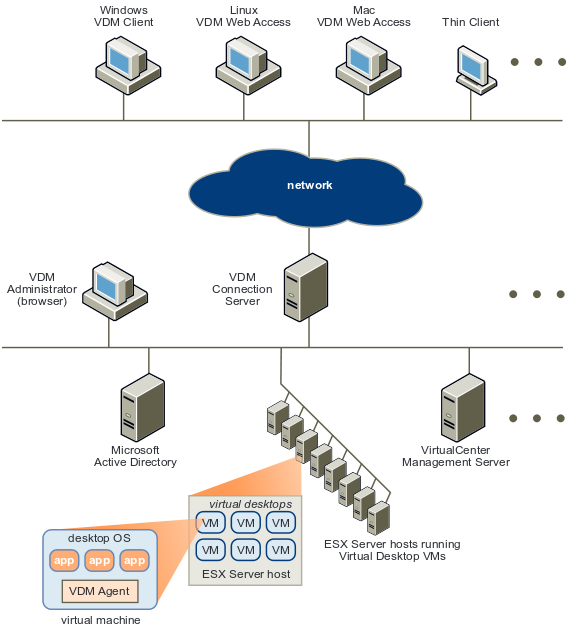
\includegraphics[width=\textwidth]{images/vmware-vdm-setup}
	\caption{\Gls{vdmLabel} Setup}
	\label{fig:vdmSetup}
\end{figure}

%cite: http://www.vmware.com/pdf/vdm20_intro.pdf

Zu Beginn werden die verschiedenen Terminals aufgelistet, mit welchen man sich auf den persönlichen Desktop verbinden kann. 

Unter der Netzwerk Wolke ist die Server Infrastruktur aufgezeigt.
Näher interessant für diese Arbeit sind die "ESX Server hosts" in der unteren Mitte. Dabei handelt es sich um virtualisierte Server welche jeder Zeit rauf- oder runter-skalliert werden können. 

Auf den ESX Hosts werden je mehrere virtuelle Desktops ausgeführt. 
Auf den Desktops kann grundsätzlich jedes Betriebsystem ausgeführt werden, für welches WMware ein VDM Agent zur Verfügung stellt.

%    Windows XP Professional with SP2 (English, Japanese, German)
%    Windows XP Professional with SP3 (English only)
%    Windows Vista Business Edition (English, Japanese, German)
%    Windows Business Ultimate Edition (English, Japanese, German)


\subsection{Kosten}
Die Berechnung der Kosten gestaltet sich schwierig, da es diverse Einflussfaktoren gibt.
VMware veröffentlichte in 2008 ein 26 seitiges Dokument mit dem Titel "Total Economic Impact Of VMware Virtual Desktop Infrastructure – Financial Services Industry" % How to link to:  https://www.vmware.com/files/pdf/analysts/Forrester_Report_Total_Economic_Impact_of_VMware_Virtual_Desktop_Infrastructure_in_Financial_Services.pdf
veröffentlicht. Darin ist ein vier Jahres Plan aufgestellt mit einer möglichen Berechnung der Kosten.

Im Dokument werden zuerst Kennzahlen, wie die Löhne und die Anzahl an Servern spezifiziert.

Als zweites werden die Initialen kosten Analysiert. Darin enthalten sind Lizenzkosten, Anzahl Arbeitsstunden sowie die Hardware welche angeschafft werden muss.

Zuletzt sind die Laufzeitkosten aufgeführt.

Im Totalen, gemäss Dokument, sind die Kosten mit \$3,648,355 beziefert. 

\begin{table}[H]
	\centering
	\small\renewcommand{\arraystretch}{1.4}  
	\rowcolors{1}{tablerowcolor}{tablebodycolor}
	%
	\captionabove[VMware \Gls{vdiLabel} Preise]{VMware \Gls{vdiLabel} Preise}
	%
	\begin{tabularx}{\textwidth}{X | r | r | r | r | r | r}
		\hline
		\rowcolor{tableheadcolor}
		\textbf{Position} & \textbf{Initial} & \textbf{Jahr 1} & \textbf{Jahr 2} & \textbf{Jahr 3} & \textbf{Jahr 4} & \textbf{Total} \\
		\hline
		Initiale Implementierungskosten & \$37,438 & \$27,038 &  &  &  & \textbf{\$64,476} \\
		Software Lizenzen und \linebreak
		Maintanance & \$9,000 & \$52,425 & \$57,188 & \$55,2425 & \$65,550 & \textbf{\$239,588} \\
		Hardware Kosten & \$365,000 & \$1,095,000 & \$680,00 & \$315,000 & \$315,000 & \textbf{\$2,770,000} \\
		Laufende Ktextbfosten für \linebreak
		Implementation und Support &  & \$137,271 & \$141,389 & \$145,631 & \$150,000 & \textbf{\$574,292} \\
		\hline
		\rowcolor{tableheadcolor}
		Total & \$411,438 & \$1,311,735 & \$878,577 & \$516,056 & \$530,550 & \textbf{\$3,648,355} \\
	\end{tabularx}
\end{table}
%Horizontale Linien sind zu lang... WIESOOO???!!!???

Mit ~76\% machen die Hardware Kosten den grössten Anteil an den totalen Kosten aus.
Das Szenario beinhaltet zu Beginn 60 Virtuelle Desktops, und wächst über die vier Jahre auf 1'000 an. Dies entspricht einer grossen Firma für welche dreieinhalb Millionen eine tragbare Investition darstellt. Für kleinere Firmen muss entsprechend runterskalliert werden.

\subsubsection{Einsparungen}
Das Paper beinhaltet auch die erwarteten Einsparungen.

\begin{table}[H]
	\centering
	\small\renewcommand{\arraystretch}{1.4}  
	\rowcolors{1}{tablerowcolor}{tablebodycolor}
	%
	\captionabove[VMware \Gls{vdiLabel} Einsparungen]{VMware \Gls{vdiLabel} Einsparungen}
	%
	\begin{tabularx}{\textwidth}{X | r | r | r | r | r}
		\hline
		\rowcolor{tableheadcolor}
		\textbf{Position} & \textbf{Jahr 1} & \textbf{Jahr 2} & \textbf{Jahr 3} & \textbf{Jahr 4} & \textbf{Total} \\
		\hline
		Outsourcing Einsparungen & \$908,160 & \$3,027,200 & \$4,540,800 & \$4,540,800 & \textbf{\$13,016,960} \\
		Help desk Einsparungen &  &  & \$239,037 & \$253,600 & \textbf{\$492,637} \\
		US contractor Einsparungen &  & \$378,400 & \$756,800 & \$1,135,200 & \textbf{\$2,270,400} \\
		Vermiedene IT Einstellungen &  &  &  & \$100,000 & \textbf{\$100,000} \\
		Vermiedene PC Anschaffungen &  & \$28,750 & \$28,700 & \$57,500 & \textbf{\$115,000} \\
		Bürofläche Einsparungen &  &  &  & \$24,000 & \textbf{\$24,000} \\
		\hline
		\rowcolor{tableheadcolor}
		Total & \$908,160 & \$3,434,350 & \$5,565,387 & \$6,111,100 & \textbf{\$16,018,997} \\
	\end{tabularx}
\end{table}

Die mit Abstand grösste Einsparung liegt mit ~82\% beim Outsourcing.

\subsubsection{Fazit}
Die genannten Zahlen sind mit einer Priese Salz zu geniessen. Als erstes wurden sie für den US Amerikanischen Markt erhoben. Zweitens sind sie sicherlich sehr optimistisch berechnet, da sie aus dem Haus von VMware selbst stammen.

Dennoch stellen die Zahlen gut dar, dass es eine grosse Investition bedeutet für die es einen guten Grund geben muss.

Aus der Einsparung-Tabelle kann man schlussfolgern, dass sich der Umschwung auf \Gls{vdiLabel} erst richtig Lohnt, wenn man auch plant Outsourcing zu betreiben. Denn ~82\% der Einsparungen beruhen auf diesem Punkt. Natürlich sind damit noch weitere Kosten verbunden die hier nicht aufgeführt sind.

\subsection{Sicherheit}
VMware integriert verschiedene Sicherheitsmassnahmen in \Gls{vdmLabel}.

\begin{itemize}
\item Zwei-Faktor-Authentifizierung
\item \Gls{httpsLabel} Zugang
\item \Gls{dmzLabel}
\item Load balancing
\item \Gls{ldapLabel}
\end{itemize}

\subsubsection{Zwei-Faktor-Authentifizierung}
\Gls{vdmLabel} unterstützt eine Zwei-Faktor-Authentifizierung mit RSA Secure ID. Beim Login muss der User Benutzername, Passwort und ein RSA Token eingeben. Dieser Vorgang ist bekannt von E-Banking Plattformen. 

Die Sicherheit besteht darin, dass wenn das Passwort in die falschen Hände gerät, sich der Angreifer nicht einloggen kann, da ihm das stetig ändernde RSA Token fehlt.

\subsubsection{\Gls{httpsLabel} Zugang}
Der Zugang von den Clients auf die \Gls{vdmLabel} Infrastruktur, sowie die Kommunikation zwischen den \Gls{vdmLabel} Servern selber kann gänzlich auf \Gls{httpsLabel} umgestellt werden.

\subsubsection{\Gls{dmzLabel} \& Load balancing}
Um den Zugriff auf die \Gls{vdiLabel} Umgebung aus dem Internet zu gewährleisten kann eine \Gls{dmzLabel} eingerichtet werden. 

\begin{figure}
	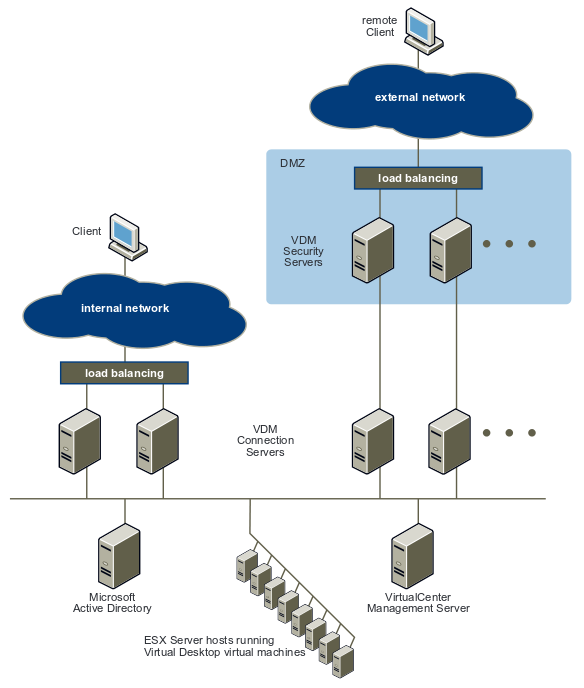
\includegraphics[width=\textwidth]{images/vmware-vdm-dmz2}
	\caption{\Gls{vdmLabel} Setup mit einer \Gls{dmzLabel}}
	\label{fig:vdmSetupDmz}
\end{figure}

Die \Gls{dmzLabel} ist ein Bereich, der vom Internet her zugänglich ist und dessen Server nicht gänzlich als vertrauenswürdig eingestuft werden können.

\Gls{vdmLabel} ermöglicht es, verschieden Security Servers einzurichten. Dabei können welche in der \Gls{dmzLabel} stehen und andere ausserhalb.

\subsubsection{Load balancing}
Um die Ausfallwahrscheinlichkeit zu minimieren, kann vor die Security Severs ein Load balancing eingeschaltet werden. Siehe Abbildung \ref{fig:vdmSetupDmz}. Dieses verteilt unter Last die Anfragen an die Server. Fällt einer aus, so merken die User, ausser eventueller Leistungseinbrüchen, nichts. 

\subsubsection{\Gls{ldapLabel}}
Die Authentifizierung kann in das \Gls{ldapLabel} der Firma integriert werden.

Dadurch wird die Benutzung vereinfacht, da die Benutzer sich mit den gewohnten Login-Daten anmelden können.

Auch die Sicherheit wird erhöht, da bei Neueintritten, internen Wechseln und Austritten die Rechte der Benutzer berücksichtigt werden.

\subsubsection{Fazit}
VMware integriert viele Sicherheit-Aspekte in ihre \Gls{vdiLabel} Lösung.

Korrekt Umgesetzt kann damit eine sichere Infrastruktur aufgebaut werden, welche robust gegenüber Ausfällen und Häckerattacken ist. Ein zusätzlicher Vorteil ist, dass die Daten in der Firma gehosted sind und die Sicherheitszone niemals verlassen.

Alles steht und fällt mit jedoch mit der Integration in die eigene Infrastruktur. Die Mechanismen müssen korrekt und durchgehen eingehalten werden damit sie effektiv sind. 

Der Zugriff über HTTP sollte durchgängig deaktiviert werden, wenn er nicht ausdrücklich benötigt wird. Sowie sollte eine sichere Firewall nach aussen hin eingerichtet sein.

\subsection{Geschwindigkeit}
% Quelle
Gemessen werden kann die Geschwindigkeit an der Latenz zwischen der Eingabe am \Gls{vdiLabel} Client bis zum Zeitpunkt wenn die Antwort auf dem Bildschirm erscheint. Als Richtwert für eine genügende Geschwindigkeit wird für eine normale Benutzung eine Sekunde vorausgesetzt, und für Ein-/Ausgabe lastige Prozesse sechs Sekunden.

\subsubsection{Testsetup}
Das Testsetup beinhaltet zwei Rechner. Der erste Rechner ist ein HP ProLiant BL460 mit einem 8-core Xeon E5540 (2.53 GHz) Prozessor und 96GB Ram. Als zweiter Rechner wurde ein Dell PowerEdge R720xd mit einem 16-core Intel Xeon E5-2690 (2.9 GHz) mit 256GB Ram verwendet.
Beide verfügen über eine \Gls{ssdLabel} mit 200GB und sechs 300GB 15k RPM SAS Festplatten.

Auf den Rechnern können beliebig viele Nodes hochgefahren werden, welche sich die Last die durch die Clients auftritt teilen.

Die Benutzer welche die Clients bedienen sind automatisiert und produzieren eine hohe Last, welche \Gls{cpuLabel} und Ein-/Ausgabe lastig ist.

Die Tests werden jeweils mit 3, 5, 8 und 16 Nodes durchgeführt. Dadurch soll ersichtlich werden, ob das System mit zunehmender Nodes- und Benutzeranzahl gut skaliert.

\subsubsection{Resultate}
Der erste Tests skalierte die Anzahl an Nodes von den definierten 3 bis zu 16 hoch und analysierte, wie viele Benutzer gleichzeitig, unter den definierten Bedinungen arbeiten konnten.

\begin{figure}
	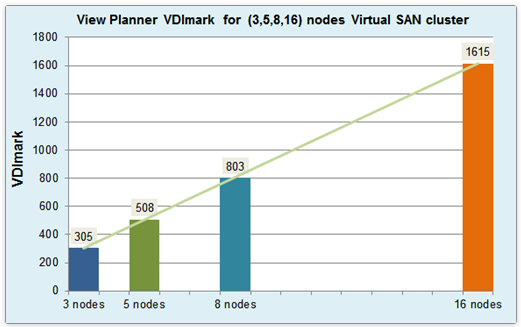
\includegraphics[width=\textwidth]{images/vmware-vdm-scale}
	\caption{Skalierung von 3 Nodes bis zu 16 Nodes}
	\label{fig:vdmPerformanceScale}
\end{figure}

Die Grafik zeigt, dass 305 Clients flüssig auf 3 Nodes arbeiten konnten. Bei 16 Nodes waren es 1615 Benutzer. Zusätzlich ist ein linearer Anstieg ersichtlich. Das heisst das System skaliert mit den Anzahl an Nodes mit.

Die zweite Grafik zeigt die Latenz für eine normale Benutzung mit der Anzahl an Benutzer aus der Abbildung \ref{fig:vdmPerformanceScale}.

\begin{figure}
	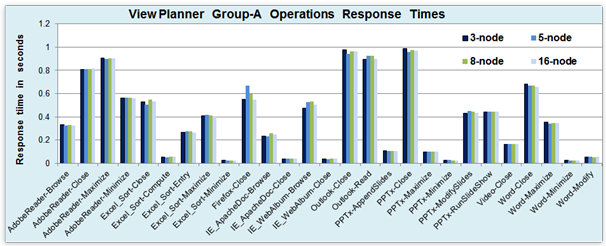
\includegraphics[width=\textwidth]{images/vmware-vdm-performance-normal}
	\caption{Antwortzeiten für normale Benutzung}
	\label{fig:vdmPerformanceNormal}
\end{figure}

Auf der letzten Grafik wird die Antwortzeit für Ein-/Ausgabe lastige Bedienung illustriert.

\begin{figure}
	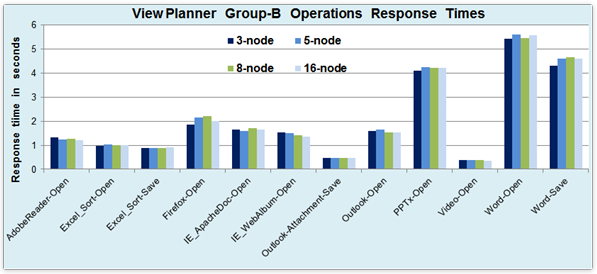
\includegraphics[width=\textwidth]{images/vmware-vdm-performance-io}
	\caption{Antwortzeiten für Ein-/Ausgabe intensive Operationen}
	\label{fig:vdmPerformanceIo}
\end{figure}

Aus den Abbildungen \ref{fig:vdmPerformanceNormal} und \ref{fig:vdmPerformanceIo} bestätigt sich, dass sich das System gleich verhaltet, wenn die Anzahl an Nodes und damit die Anzahl an Clients erhöht wird.

\subsubsection{Fazit}
Mit genug starker Hardware kann jede gewünschte Antwortzeit erreicht werden. Bei VMwares \Gls{vdmLabel} Lösung sind das durchschnittlich 101 Benutzer pro Node mit einer Toleranz von einer beziehungsweise sechs Sekunden.

Das spannendste ist jedoch die lineare Entwicklung mit zunehmender Nodeanzahl. Damit ist das System für kleinere Firmen gleich gut geeignet wie für grosse.

\subsection{Produkt Lösungen}





